\documentclass[14pt,a4paper]{extarticle}
\usepackage[T2A]{fontenc}
\usepackage[utf8]{inputenc}
\usepackage[english,russian]{babel}
\usepackage{lmodern}
\usepackage{geometry}
\usepackage{array}
\usepackage{tabularx}
\usepackage{longtable}
\usepackage{ltablex}
\usepackage{booktabs}
\usepackage{hyperref}
\usepackage{indentfirst}
\usepackage{microtype}
\usepackage{graphicx}
\usepackage{setspace}
\usepackage{listings}
\usepackage{graphicx}
\usepackage{caption}
\usepackage{float}
\usepackage{tocloft}
\usepackage{titlesec}
\usepackage{newtxtext,newtxmath}

\titleformat{\section}        % форматируем \section
  {\normalfont\bfseries}      % стиль: обычный + жирный
  {\thesection.}              % номер секции с точкой
  {2mm}                       % расстояние между номером и текстом
  {}                           % перед заголовком можно добавить что-то
\titlespacing*{\section}{1.5cm}{*3}{*1}  % {отступ слева}{отступ сверху}{отступ снизу}

\titleformat{\subsection}        % форматируем \section
  {\normalfont\bfseries}      % стиль: обычный + жирный
  {\thesubsection.}              % номер секции с точкой
  {2mm}                       % расстояние между номером и текстом
  {}                           % перед заголовком можно добавить что-то
\titlespacing*{\subsection}{1.5cm}{*3}{*1}  % {отступ слева}{отступ сверху}{отступ снизу}

\captionsetup{justification=centering}
\renewcommand{\ttdefault}{cmtt}
\keepXColumns
\setlength{\parindent}{3em}
\newgeometry{left=2.5cm,right=2.5cm,top=3cm,bottom=2.5cm}

\renewcommand{\contentsname}{\hspace*{4em}{\smallСодержание}}
\setlength{\cftbeforesecskip}{0.5em}
\renewcommand{\cftsecleader}{\cftdotfill{\cftdotsep}}
\renewcommand{\cftsecaftersnum}{.\hspace{2mm}}

\title{Отчёт по "Управление ИТ-проектами"}
\author{Выполнил студент группы М-РИТ-25-1, Станиславчук Сергей}

\begin{document}

\setstretch{1.5}
\noindent
\begin{minipage}[t]{0.01\textwidth}
    \includegraphics{~/programmer/++Programmer/5_1/LSTU.jpg}
\end{minipage}%
\begin{minipage}[c]{1.1\linewidth}
    \centering
    {\small
    МИНИСТЕРСТВО НАУКИ И ВЫСШЕГО ОБРАЗОВАНИЯ РФ \\[1em]
    ФЕДЕРАЛЬНОЕ ГОСУДАРСТВЕННОЕ БЮДЖЕТНОЕ \\
    ОБРАЗОВАТЕЛЬНОЕ УЧРЕЖДЕНИЕ ВЫСШЕГО ОБРАЗОВАНИЯ \\
    «ЛИПЕЦКИЙ ГОСУДАРСТВЕННЫЙ ТЕХНИЧЕСКИЙ УНИВЕРСИТЕТ»
    }
\end{minipage}%

\vspace{3em}

\noindent
\hspace{1em}%
\begin{minipage}[t]{0.8\textwidth}
\textbf{Институт} \hspace{2em} компьютерных наук \\
\textbf{Кафедра} \hspace{2em} автоматизированных систем управления
\end{minipage}


\vspace{6em}

\begin{center}
\textbf{Лабораторная работа №1} \\
по дисциплине \\ <<Нейронные сети и глубокое обучение>>
\end{center}

\vspace{6em}

\noindent
\begin{tabular*}{\textwidth}{@{\extracolsep{\fill}} l c r }
    Студент М-РИТ-25-1 & \makebox[4cm]{\hrulefill} & Станиславчук С.М. \\[2em]
Руководитель & \\
Профессор & \makebox[4cm]{\hrulefill} & Седых И.А. \\
\end{tabular*}

\vfill
\begin{center}
    Липецк, 2026
\end{center}

\thispagestyle{empty}

\newpage
\tableofcontents
\newpage

\section{Выдача задания}

 В рамках лаборатной работы поставлена задача обучения многослойного
 перцептрона с алгоритмом обратного распространения ошибки.

Вариант 17:
Функция
\begin{verbatim}

import numpy as np
np.random.seed(17)
X = np.random.uniform(0, 4*np.pi, 600).reshape(-1, 1)
y = np.sin(X) + 0.3*np.sin(5*X) + np.random.normal(0, 0.1, X.shape)

\end{verbatim}

Активация скрытых слоев: ReLU; архитектура: Вход(1) -> 64 -> 32 -> Выход(1, Linear)

\section{Ход работы}

В качестве метрики определяющей точность использую MSE.
Скорость обучения для всех функций активации постоянна = 0.02

\subsection{ReLU + ReLU}

\begin{verbatim}
epoch 0, loss 1.136373
epoch 200, loss 0.215445
epoch 400, loss 0.169322
epoch 600, loss 0.162735
Test MSE: 0.18996727415942807
\end{verbatim}

График потерь и сравнения ReLU + ReLU приведены на рис. 1, 2.
\begin{figure}[H]
    \label{fig:pic1}
    \centering
    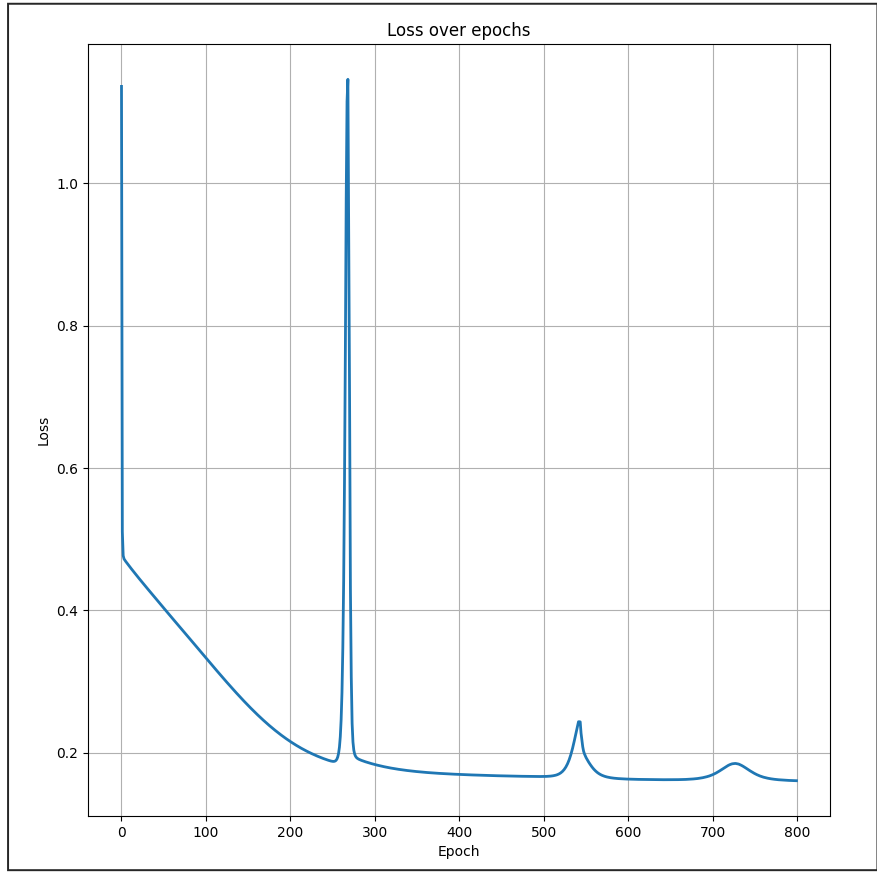
\includegraphics[width=0.78\textwidth]{rr/loss.png}
    \refstepcounter{figure}
    \caption*{Рисунок \thefigure\ — Потери (ReLU + ReLU)}
\end{figure}

\begin{figure}[H]
    \label{fig:pic2}
    \centering
    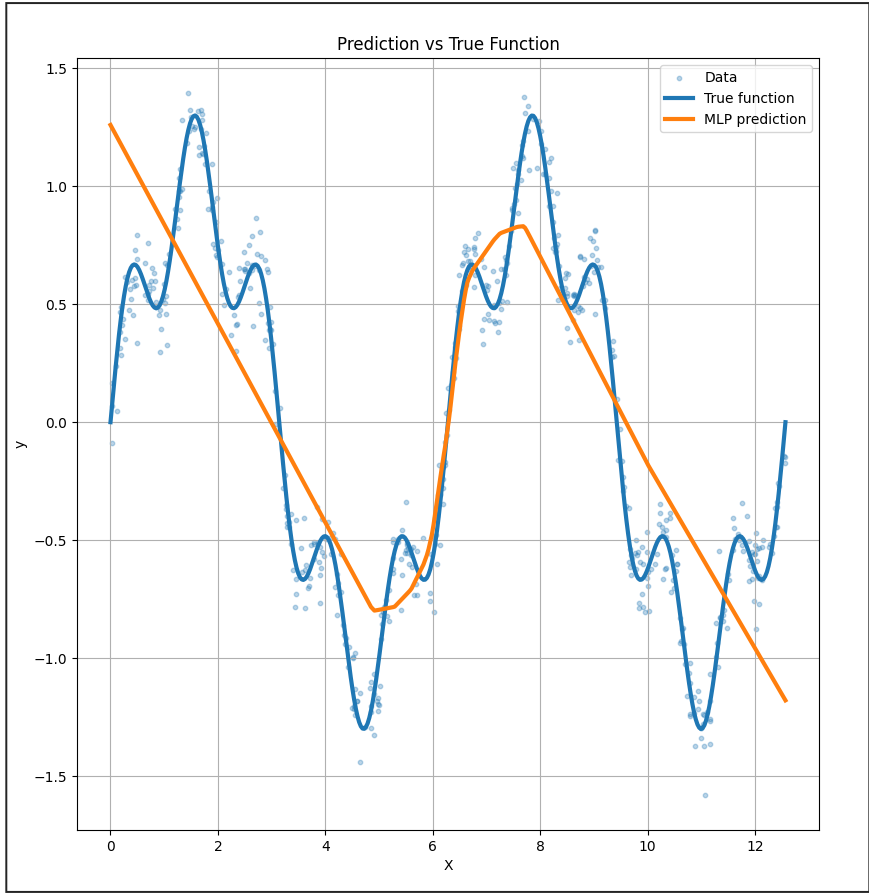
\includegraphics[width=0.78\textwidth]{rr/comp.png}
    \refstepcounter{figure}
    \caption*{Рисунок \thefigure\ — Сравнение с исходной (ReLU + ReLU)}
\end{figure}

\subsection{ReLU + Tanh}

\begin{verbatim}
epoch 0, loss 0.645922
epoch 200, loss 0.131175
epoch 400, loss 0.121557
epoch 600, loss 0.116986
Test MSE: 0.1320729197341313
\end{verbatim}

График потерь и сравнения ReLU + Tanh приведены на рис. 3, 4.
\begin{figure}[H]
    \label{fig:pic3}
    \centering
    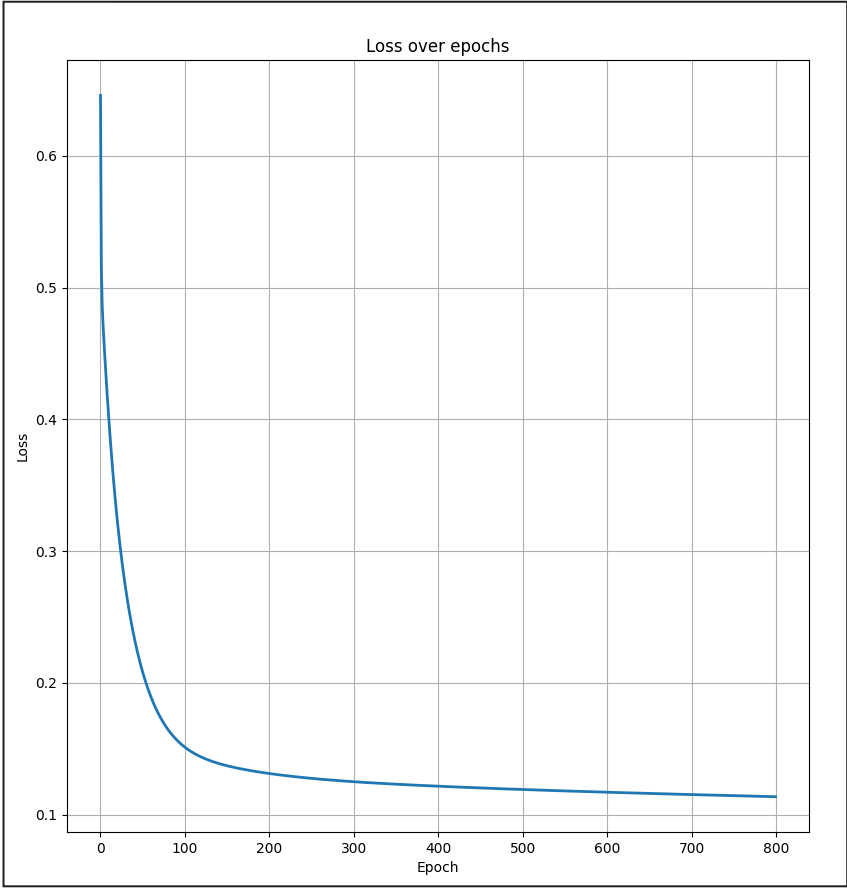
\includegraphics[width=0.78\textwidth]{rt/loss.png}
    \refstepcounter{figure}
    \caption*{Рисунок \thefigure\ — Потери (ReLU + Tanh)}
\end{figure}

\begin{figure}[H]
    \label{fig:pic4}
    \centering
    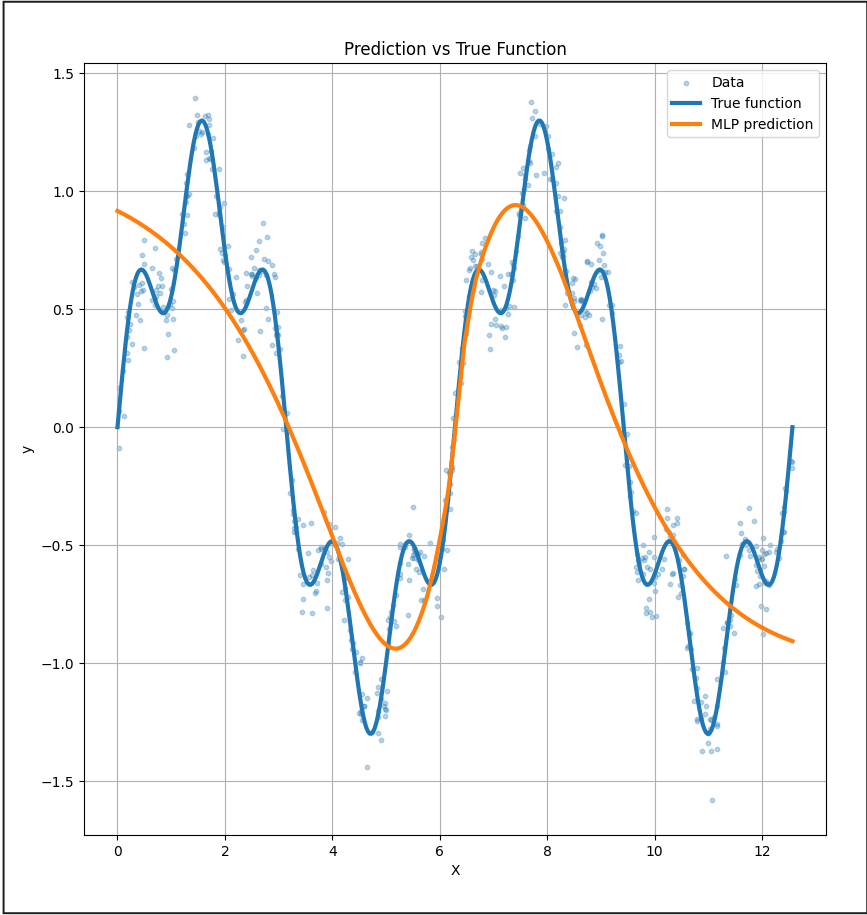
\includegraphics[width=0.78\textwidth]{rt/comp.png}
    \refstepcounter{figure}
    \caption*{Рисунок \thefigure\ — Сравнение с исходной (ReLU + Tanh)}
\end{figure}

\subsection{ReLU + Sigmoid}

\begin{verbatim}
epoch 0, loss 0.662178
epoch 200, loss 0.431442
epoch 400, loss 0.323692
epoch 600, loss 0.219722
Test MSE: 0.1567918362202583
\end{verbatim}

График потерь и сравнения ReLU + Sigmoid приведены на рис. 5, 6.
\begin{figure}[H]
    \label{fig:pic3}
    \centering
    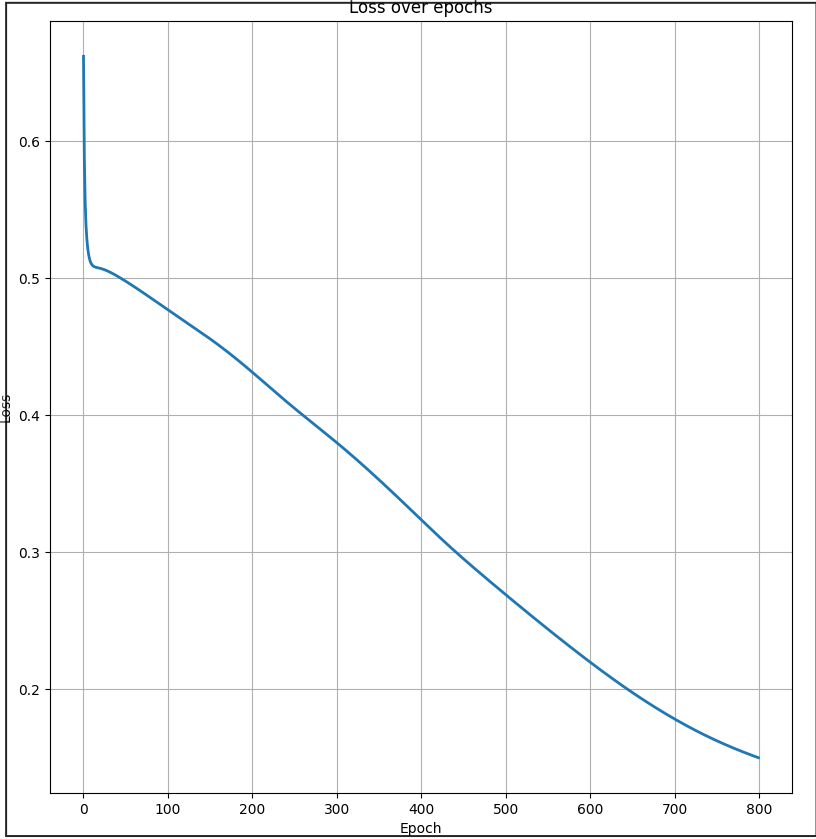
\includegraphics[width=0.78\textwidth]{rs/loss.png}
    \refstepcounter{figure}
    \caption*{Рисунок \thefigure\ — Потери (ReLU + Sigm)}
\end{figure}

\begin{figure}[H]
    \label{fig:pic4}
    \centering
    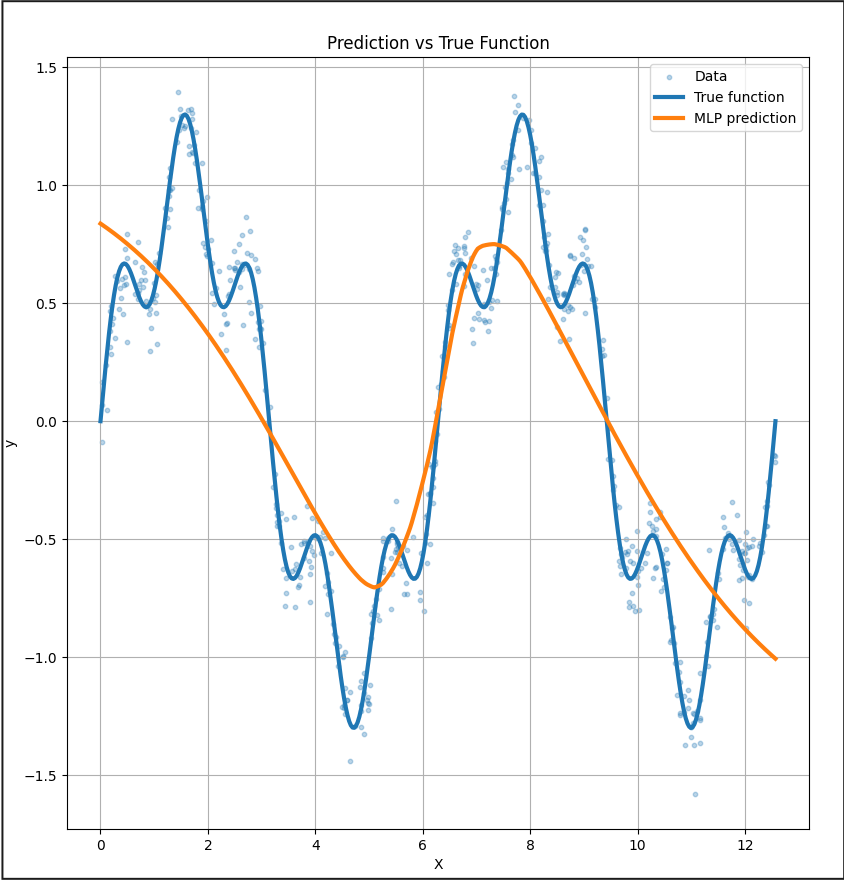
\includegraphics[width=0.78\textwidth]{rs/comp.png}
    \refstepcounter{figure}
    \caption*{Рисунок \thefigure\ — Сравнение с исходной (ReLU + Sigm)}
\end{figure}

\section{Вывод}
В ходе лабораторной работы была проведена сравнительная оценка трёх конфигураций многослойного перцептрона, различающихся выбором функций активации: ReLU+ReLU, ReLU+Tanh и ReLU+Sigmoid. Целевая функция представляла собой суперпозицию синусоид, что накладывает требования на способность модели аппроксимировать гладкие, знакопеременные и периодические зависимости.

Результаты обучения показали, что наилучшее качество аппроксимации достигается при использовании комбинации ReLU на первом скрытом слое и гиперболического тангенса на втором. Это объясняется тем, что функция ReLU эффективно выполняет первичное преобразование признаков, формируя кусочно-линейное представление входного пространства без эффекта насыщения в положительной области. В свою очередь, функция Tanh является симметричной относительно нуля и обладает гладкой нелинейностью, что позволяет корректно моделировать знакопеременную природу целевой функции и её кривизну.

Конфигурация ReLU+ReLU показала худшие результаты, несмотря на стабильное снижение функции потерь. Это связано с тем, что композиция функций ReLU формирует исключительно кусочно-линейное приближение. Для аппроксимации периодических функций в таком случае требуется значительно большее число нейронов, поскольку модель вынуждена воспроизводить гладкую кривую через ломаную структуру.

Использование сигмоидальной функции активации во втором слое (ReLU+Sigmoid) также привело к ухудшению качества обучения. Основной причиной является эффект насыщения сигмоиды, при котором производная функции стремится к нулю на больших по модулю значениях аргумента. Это приводит к затуханию градиентов и замедлению процесса оптимизации. Дополнительно сигмоида не является симметричной относительно нуля, что усложняет моделирование знакопеременных зависимостей.

Таким образом, комбинация ReLU и Tanh обеспечивает наиболее адекватное соответствие архитектуры сети свойствам целевой функции. ReLU формирует базовое представление данных, тогда как Tanh обеспечивает необходимую нелинейность для аппроксимации гладких колебательных процессов. Полученные результаты согласуются с теоретическими представлениями о влиянии функций активации на выразительную способность нейронных сетей и динамику их обучения.
\end{document}
